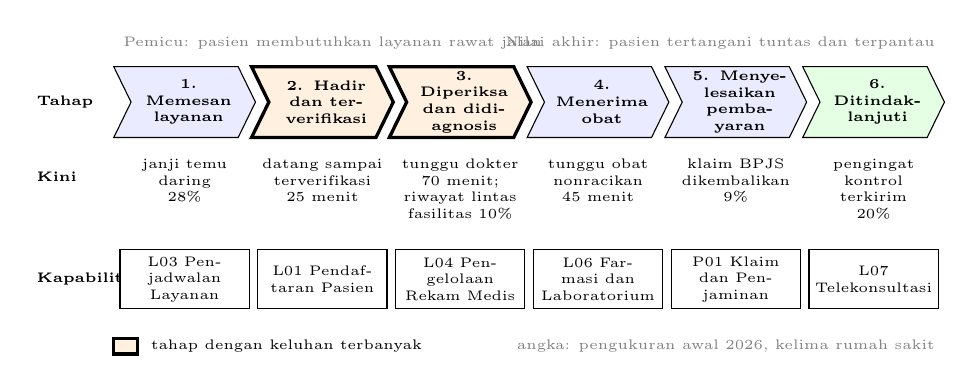
\begin{tikzpicture}[
  font=\scriptsize,
  tahap/.style={fill=blue!8, draw},
  tekan/.style={fill=orange!12, draw, very thick},
  isi/.style={text width=1.25cm, align=center, font=\tiny\bfseries},
  ukur/.style={text width=1.6cm, align=center, font=\tiny, anchor=north},
  kap/.style={draw, fill=white, text width=1.5cm, minimum height=0.75cm,
              align=center, font=\tiny, inner sep=2pt},
  label/.style={font=\tiny\bfseries, anchor=west}
]
  \node[font=\tiny, gray, anchor=west] at (1.1,1.2)
    {Pemicu: pasien membutuhkan layanan rawat jalan};
  \node[font=\tiny, gray, anchor=east] at (11.65,1.2)
    {Nilai akhir: pasien tertangani tuntas dan terpantau};

  \node[label] at (0,0.45) {Tahap};
  \node[label] at (0,-0.5) {Kini};
  \node[label] at (0,-1.8) {Kapabilitas};

  \draw[tahap] (1.10,0) -- ++(1.58,0) -- ++(0.22,0.45) -- ++(-0.22,0.45)
    -- ++(-1.58,0) -- ++(0.22,-0.45) -- cycle;
  \draw[tekan] (2.85,0) -- ++(1.58,0) -- ++(0.22,0.45) -- ++(-0.22,0.45)
    -- ++(-1.58,0) -- ++(0.22,-0.45) -- cycle;
  \draw[tekan] (4.60,0) -- ++(1.58,0) -- ++(0.22,0.45) -- ++(-0.22,0.45)
    -- ++(-1.58,0) -- ++(0.22,-0.45) -- cycle;
  \draw[tahap] (6.35,0) -- ++(1.58,0) -- ++(0.22,0.45) -- ++(-0.22,0.45)
    -- ++(-1.58,0) -- ++(0.22,-0.45) -- cycle;
  \draw[tahap] (8.10,0) -- ++(1.58,0) -- ++(0.22,0.45) -- ++(-0.22,0.45)
    -- ++(-1.58,0) -- ++(0.22,-0.45) -- cycle;
  \draw[tahap, fill=green!10] (9.85,0) -- ++(1.58,0) -- ++(0.22,0.45)
    -- ++(-0.22,0.45) -- ++(-1.58,0) -- ++(0.22,-0.45) -- cycle;

  \node[isi] at (2.05,0.45) {1. Memesan layanan};
  \node[isi] at (3.80,0.45) {2. Hadir dan terverifikasi};
  \node[isi] at (5.55,0.45) {3. Diperiksa dan didiagnosis};
  \node[isi] at (7.30,0.45) {4. Menerima obat};
  \node[isi] at (9.05,0.45) {5. Menyelesaikan pembayaran};
  \node[isi] at (10.80,0.45) {6. Ditindak\-lanjuti};

  \node[ukur] at (2.00,-0.15) {janji temu daring\\28\%};
  \node[ukur] at (3.75,-0.15) {datang sampai terverifikasi\\25 menit};
  \node[ukur] at (5.50,-0.15) {tunggu dokter 70 menit; riwayat lintas fasilitas 10\%};
  \node[ukur] at (7.25,-0.15) {tunggu obat nonracikan\\45 menit};
  \node[ukur] at (9.00,-0.15) {klaim BPJS dikembalikan\\9\%};
  \node[ukur] at (10.75,-0.15) {pengingat kontrol terkirim\\20\%};

  \node[kap] at (2.00,-1.8) {L03 Penjadwalan Layanan};
  \node[kap] at (3.75,-1.8) {L01 Pendaftaran Pasien};
  \node[kap] at (5.50,-1.8) {L04 Pengelolaan Rekam Medis};
  \node[kap] at (7.25,-1.8) {L06 Farmasi dan Laboratorium};
  \node[kap] at (9.00,-1.8) {P01 Klaim dan Penjaminan};
  \node[kap] at (10.75,-1.8) {L07 Telekonsul\-tasi};

  \draw[fill=orange!12, very thick] (1.1,-2.55) rectangle (1.4,-2.75);
  \node[font=\tiny, anchor=west] at (1.45,-2.65) {tahap dengan keluhan terbanyak};
  \node[font=\tiny, gray, anchor=east] at (11.65,-2.65)
    {angka: pengukuran awal 2026, kelima rumah sakit};
\end{tikzpicture}
